

\documentclass{beamer}
\usepackage{etex}

\usetheme[secheader]{Madrid} 
\usecolortheme{beaver}
\setbeamercolor*{palette primary}{fg=darkred!60!black,bg=gray!10!white}
\setbeamercolor{frametitle}{bg=gray!10!white}
\usefonttheme{serif}

\usepackage{textpos}
\usepackage{pstricks}
\usepackage{pstricks-add}
\usepackage{xcolor}
\usepackage{amssymb}
\usepackage{pifont}
\usepackage{tabularx}
\usepackage{tabulary}


\title{o-Minimality and its Variations}
\author[Vagios Vlachos]{Vagios Vlachos}
\institute[$\mu\Pi\lambda\forall$]{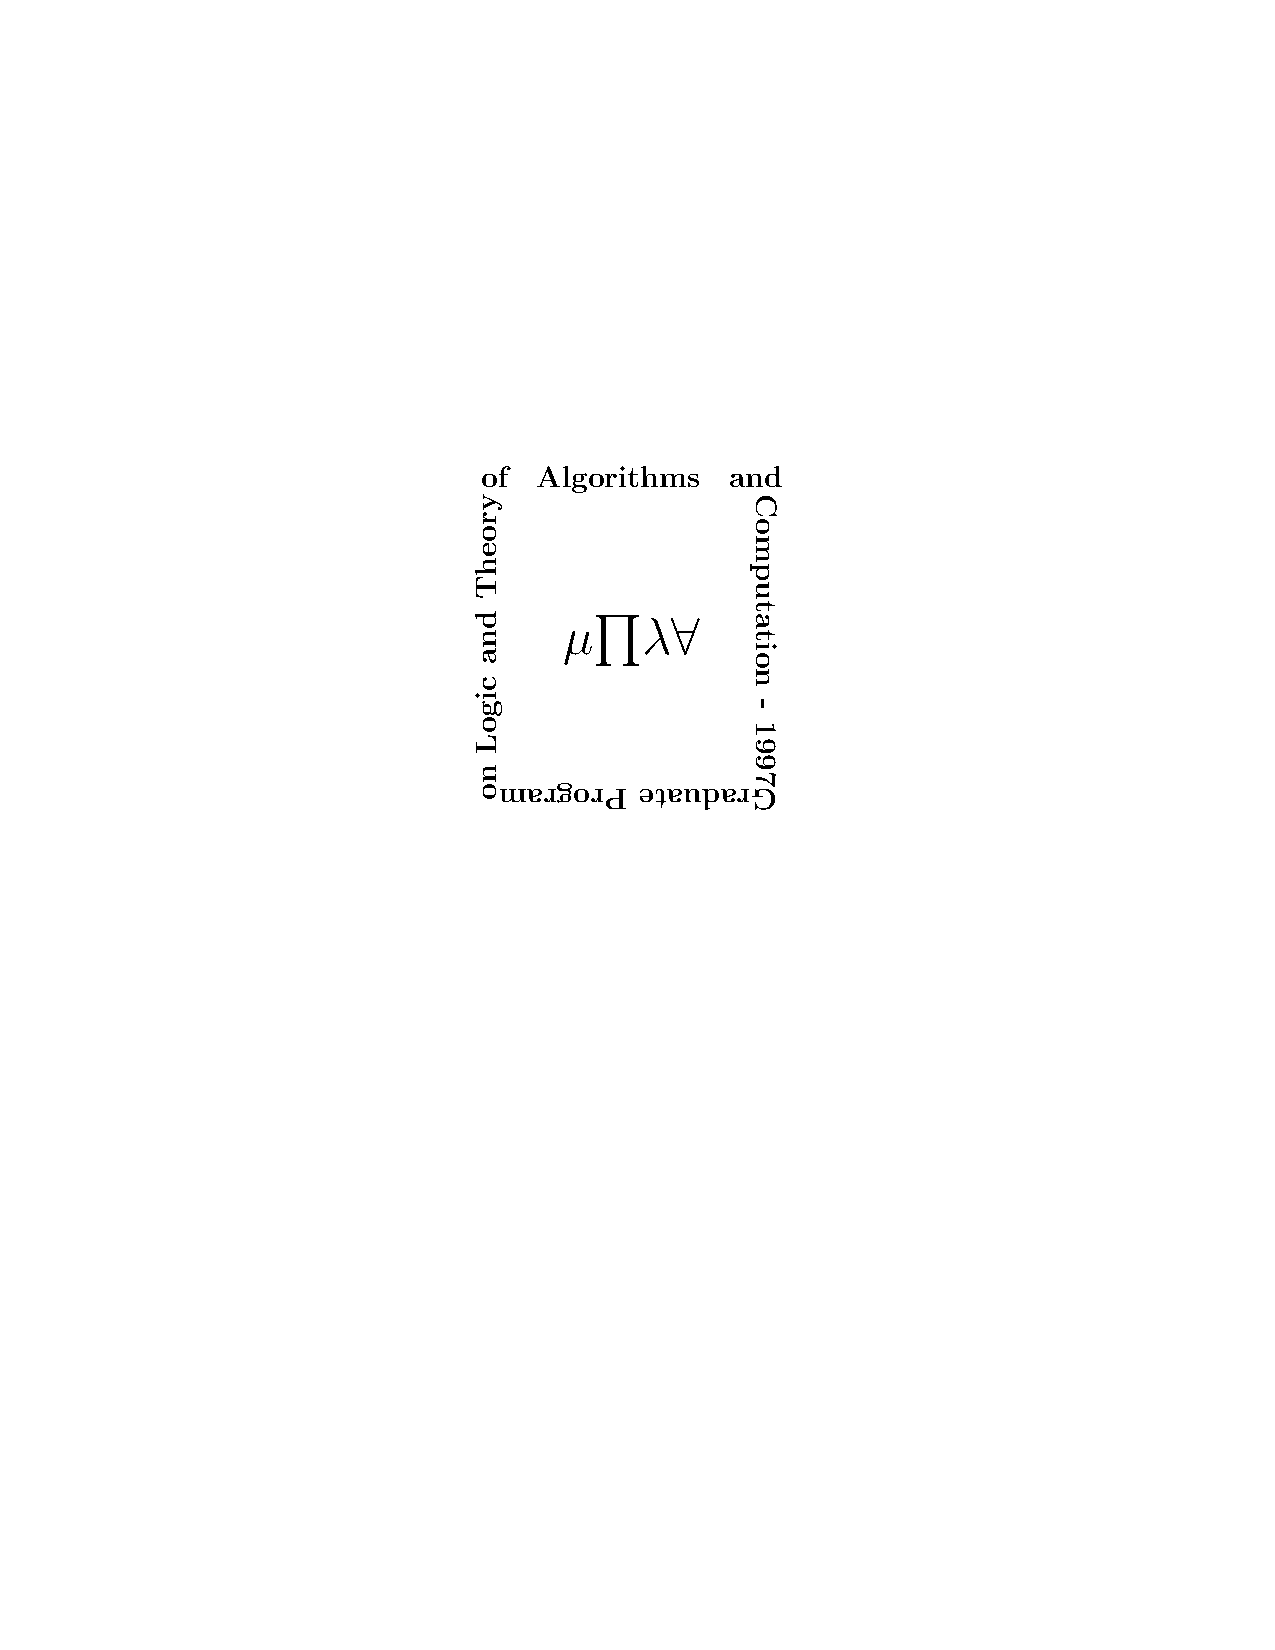
\includegraphics[height=2cm,width=2cm]{mpla-logo-.pdf}\\Graduate Program on Login and Theory of Algorithms and Computation}
\date[]{2014}


\begin{document}

\begin{frame}
  \maketitle
\end{frame}

\addtobeamertemplate{frametitle}{}{%
\begin{textblock*}{100mm}(.90\textwidth,-1.37cm)
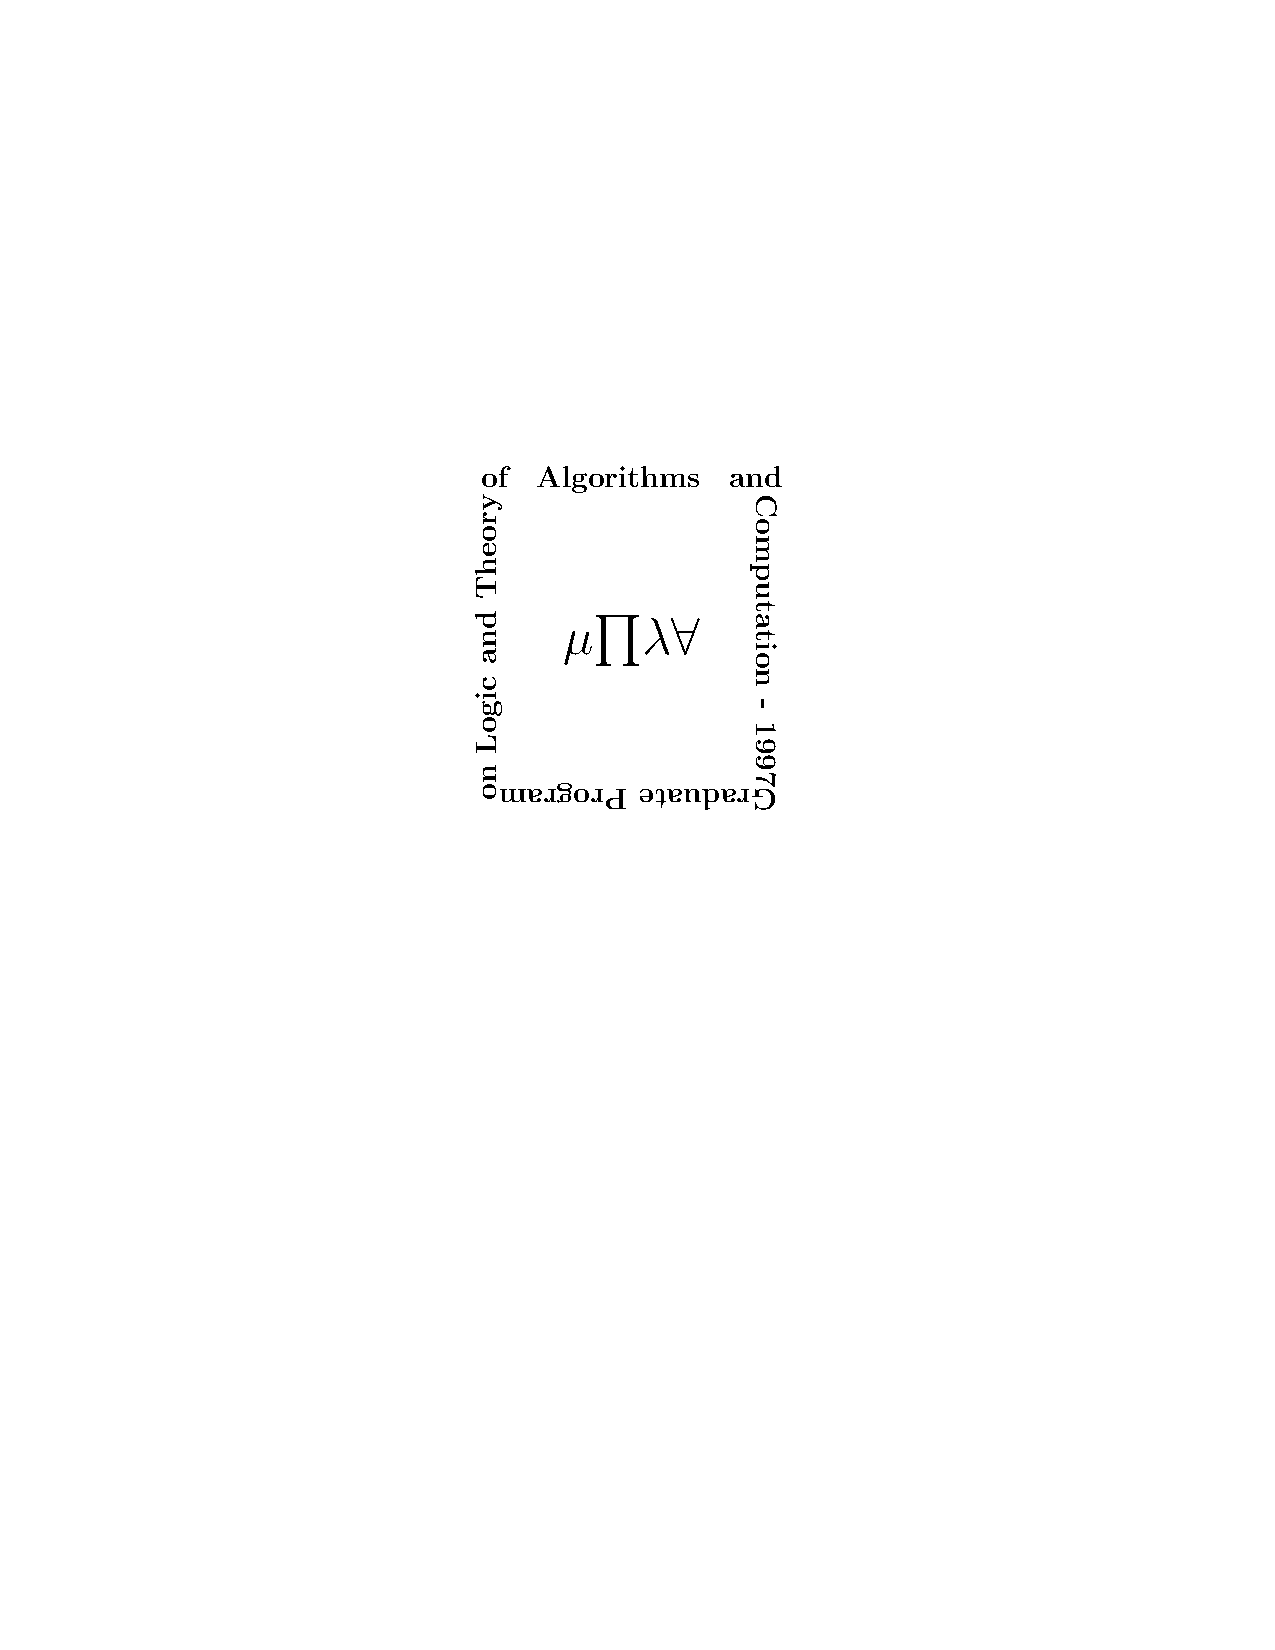
\includegraphics[height=1.4cm,width=1.4cm]{mpla-logo-.pdf}
\end{textblock*}}

%!TEX root = main.tex

\section{o-Minimality}
\subsection{Introduction}


\begin{frame}[c]{o-Minimality}
	\begin{block}{Assumptions}
		\begin{itemize}
			\item $\mathcal{M}=(M,<,\ldots)$
			\item $<$ is dense, linear, without endpoints
			\item definability with parameters
		\end{itemize}
	\end{block}

	\begin{definition}
		The structure $\mathcal{M}$ is called \em o-minimal \em if every definable subset of $M$ is a finite union of singletons and open intervals with endpoints in $M_{\infty}:=M\cup\{-\infty,+\infty\}$.\\
		A theory $T$ is called \em o-minimal \em if every model $\mathcal{M}$ of $T$ is o-minimal.
	\end{definition}
\end{frame}

\begin{frame}[c]{o-Minimality}
	The class of o-minimal structures is,
		\begin{itemize}
			\item closed under reducts (if $<$ still remains in the language)
			\item closed under expansions by constants
		\end{itemize}

	\begin{exampleblock}{Some o-minimal structures}
		\begin{itemize}
			\item $(\mathbb{Q},<)$
			\item $(\mathbb{Q},<,+)$
			\item $\mathcal{R}=(\mathbb{R},<,+,-,\cdot,0,1)$
		\end{itemize}
	\end{exampleblock}

	\begin{block}{$(\mathbb{Q},<,+,\cdot,0,1)$ is not o-minimal}
		The infinite discrete set of perfect squares is definable.
	\end{block}
\end{frame}

\subsection{Monotonicity and Finiteness}

\begin{frame}[c]{Monotonicity and Finiteness}
	\begin{block}{Monotonicity Theorem}
		Let $\mathcal{M}$ be an o-minimal structure and $f:(a,b) \to M$ be a definable function with domain $(a,b)$(possibly $a=- \infty$ or $b=+ \infty$).
		Then, there are points $a=a_0<a_1< \cdots <a_{k+1}$ s.t. for each $j=0,\ldots,k$, $f|_{(a_j,a_{j+1})}$ is either,
		\begin{itemize}
			\item constant, or
			\item a strictly monotonic and continuous bijection to an interval.
		\end{itemize}
 	\end{block}
 	% The proof of this utilizes the following lemma.
 	% \begin{block}{Lemma}
 	% 	Let $f$ be a function as described in the Monotonicity Theorem.
 	% 	Then for any definable infinite interval $I \subseteq (a,b)$, there is an infinite $I^* \subseteq I$ on which $f$ is either constant or strictly monotone.
 	% \end{block}

 	\begin{beamerboxesrounded}[shadow=true]{Finiteness Lemma}
 		Let $A \subseteq M^2$ be definable and suppose that for each $x \in M$ the fiber $A_x := \{ y \in M|(x,y) \in A \}$ is finite.
		Then there is $N < \omega$ s.t. $|A_x| \leq N$ for all $x \in M$. 
 	\end{beamerboxesrounded}
\end{frame}

% \begin{frame}[t]\frametitle{Proof of Monotonicity Theorem}
%     Conside the formula $\theta(x)$
%     \begin{beamerboxesrounded}[shadow=true]{}
%     	``On an interval of which $x$ is the left endpoint, $f$ is strictly monotone or constant, and there is no interval extending this interval on the left on which $f$ is strictly monotone or constant.''
%     \end{beamerboxesrounded}
% \end{frame}

\begin{frame}[c]\frametitle{Applications}	
    
	\begin{block}{Corollary}
		Let $f:(a,b) \to M$ be definale and continuous. Then $f$ takes a maximum and minimum value on $[a,b]$.
	\end{block}

	\begin{block}{Exchange Principle}
		Let $\mathcal{M}$ be o-minimal.
		Let $b,c,a_1,\ldots,a_n \in \mathcal{M}$.
		If $b$ is definable over $c,a_1,\ldots,a_n$, and $b$ is not definable over $a_1,\ldots,a_n$, then $c$ is definable over $b,a_1,\ldots,a_n$.
	\end{block}

\end{frame}

\subsection{Cell Decomposition}

\begin{frame}[c]\frametitle{Motivation}
	
	\begin{beamerboxesrounded}[shadow=true, upper=question]{Question}
		What happens with the definable subsets of $M^n$?
	\end{beamerboxesrounded}
    
	\begin{beamerboxesrounded}[shadow=true]{Notation}
		Given definable $X \subseteq M^n$
		\begin{itemize}
			\item $C(X):= \{ f:X \to M|f \text{ is definable and continuous}\}$
			\item $C_\infty(X):=C(X) \cup \{ -\infty, +\infty \}$
			\item for $f,g \in C_\infty(X)$ s.t. $(\forall \bar{x} \in X)(f(\bar{x})<g(\bar{x}))$ then 
			$$(f,g)_X := \{  (\bar{x},y)\in X \times M|f(\bar{x})<y<g(\bar{x})\}$$
		\end{itemize}
	\end{beamerboxesrounded}

\end{frame}

\begin{frame}[c]\frametitle{Cells}

		Let $(i_1,\ldots,i_n)$ be a binary sequence. Then a $(i_1,\ldots,i_n)$-\em cell \em is a definable subset of $M^n$ defined as follows,
		\begin{columns}

			\begin{column}{7cm}
					\begin{itemize}
						\item a $(0)$-cell is a singleton
						\item a $(1)$-cell is an open interval
					\end{itemize}
					Suppose that we have defined $(i_1,\ldots,i_{n-1})$-cells, then
					\begin{itemize}
						\item<2-> a $(i_1,\ldots,i_{n-1},0)$-cell is the graph of some $f \in C(X)$,
						where $X$ is a  $(i_1,\ldots,i_{n-1})$-cell
						\item<3-> a $(i_1,\ldots,i_{n-1},1)$-cell is the set $(f,g)_X$ where $X$ is a
						$(i_1,\ldots,i_{n-1})$-cell and $f,g \in C_\infty(X)$
					\end{itemize}

			\end{column}

			\begin{column}{4cm}

				\temporal<2>{}{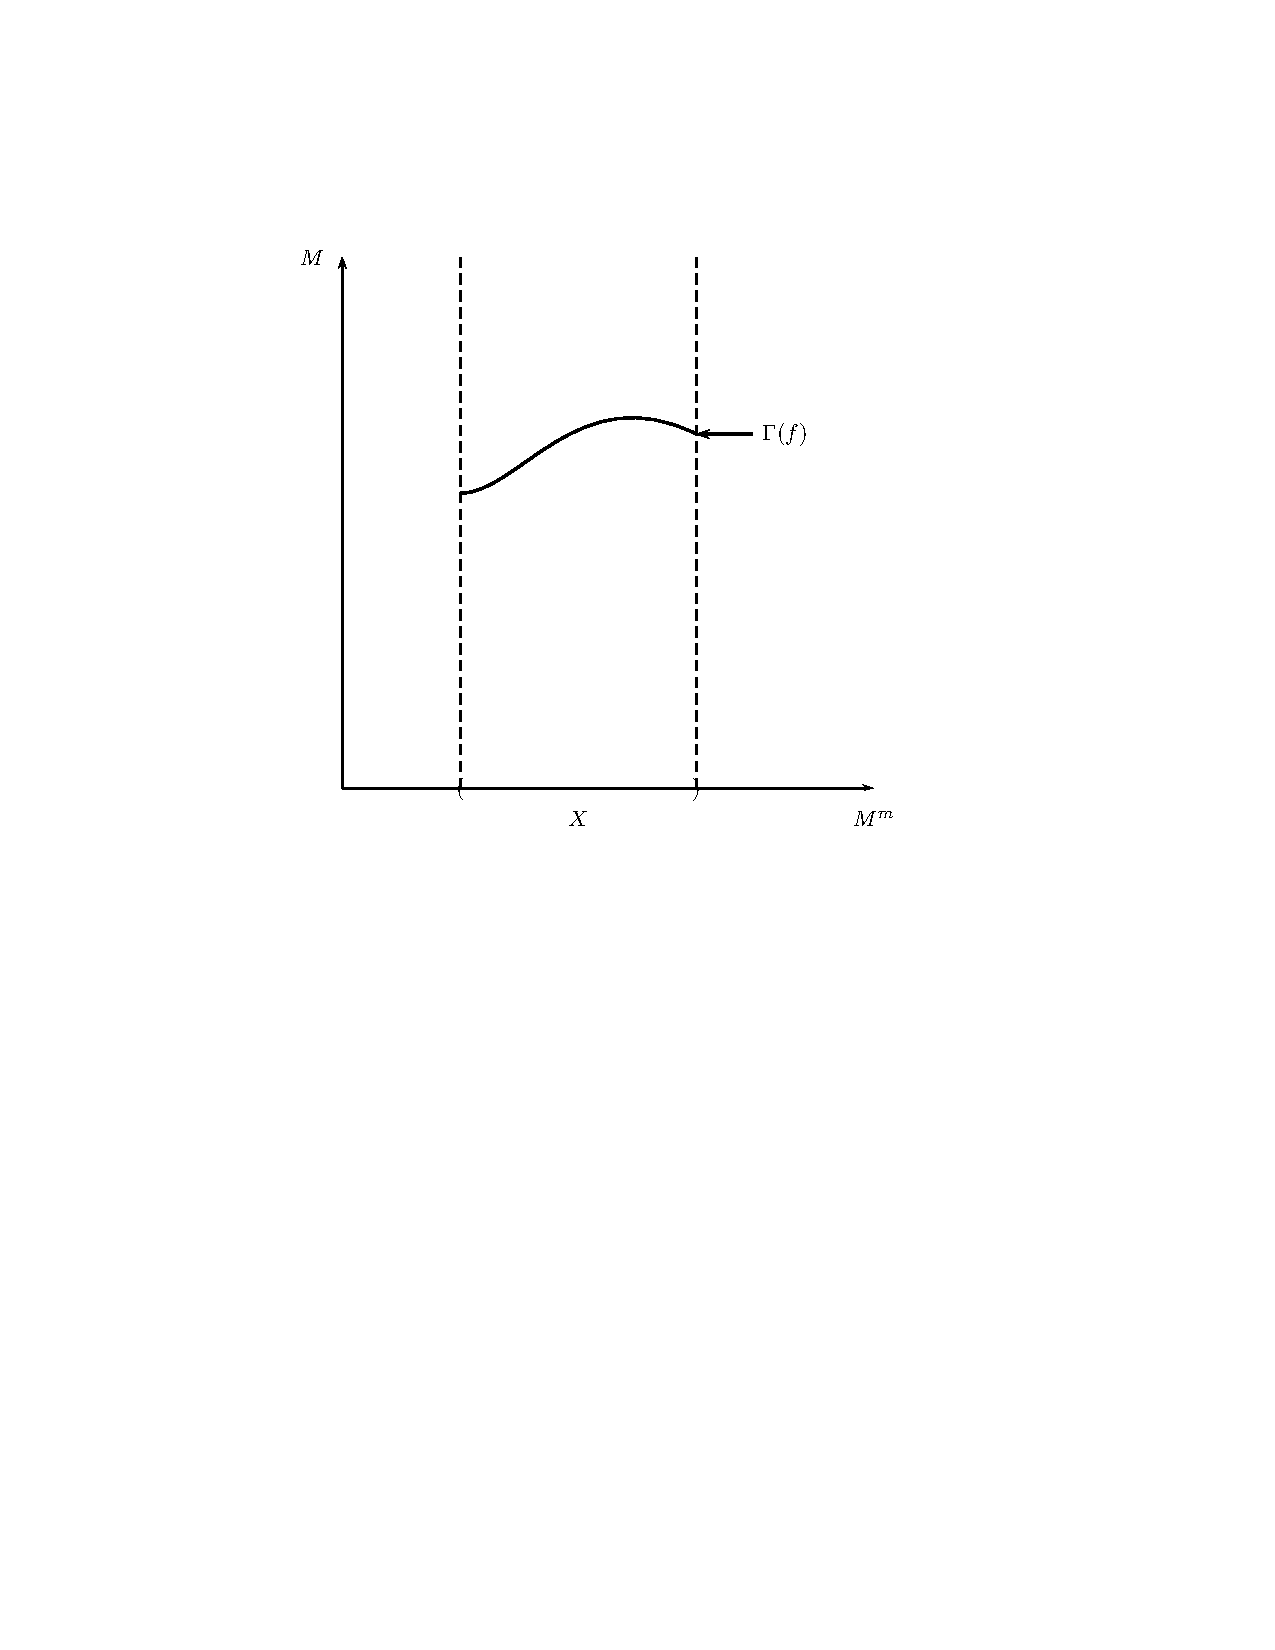
\includegraphics[height=5cm,width=4cm]{img/celliii0-.pdf}}{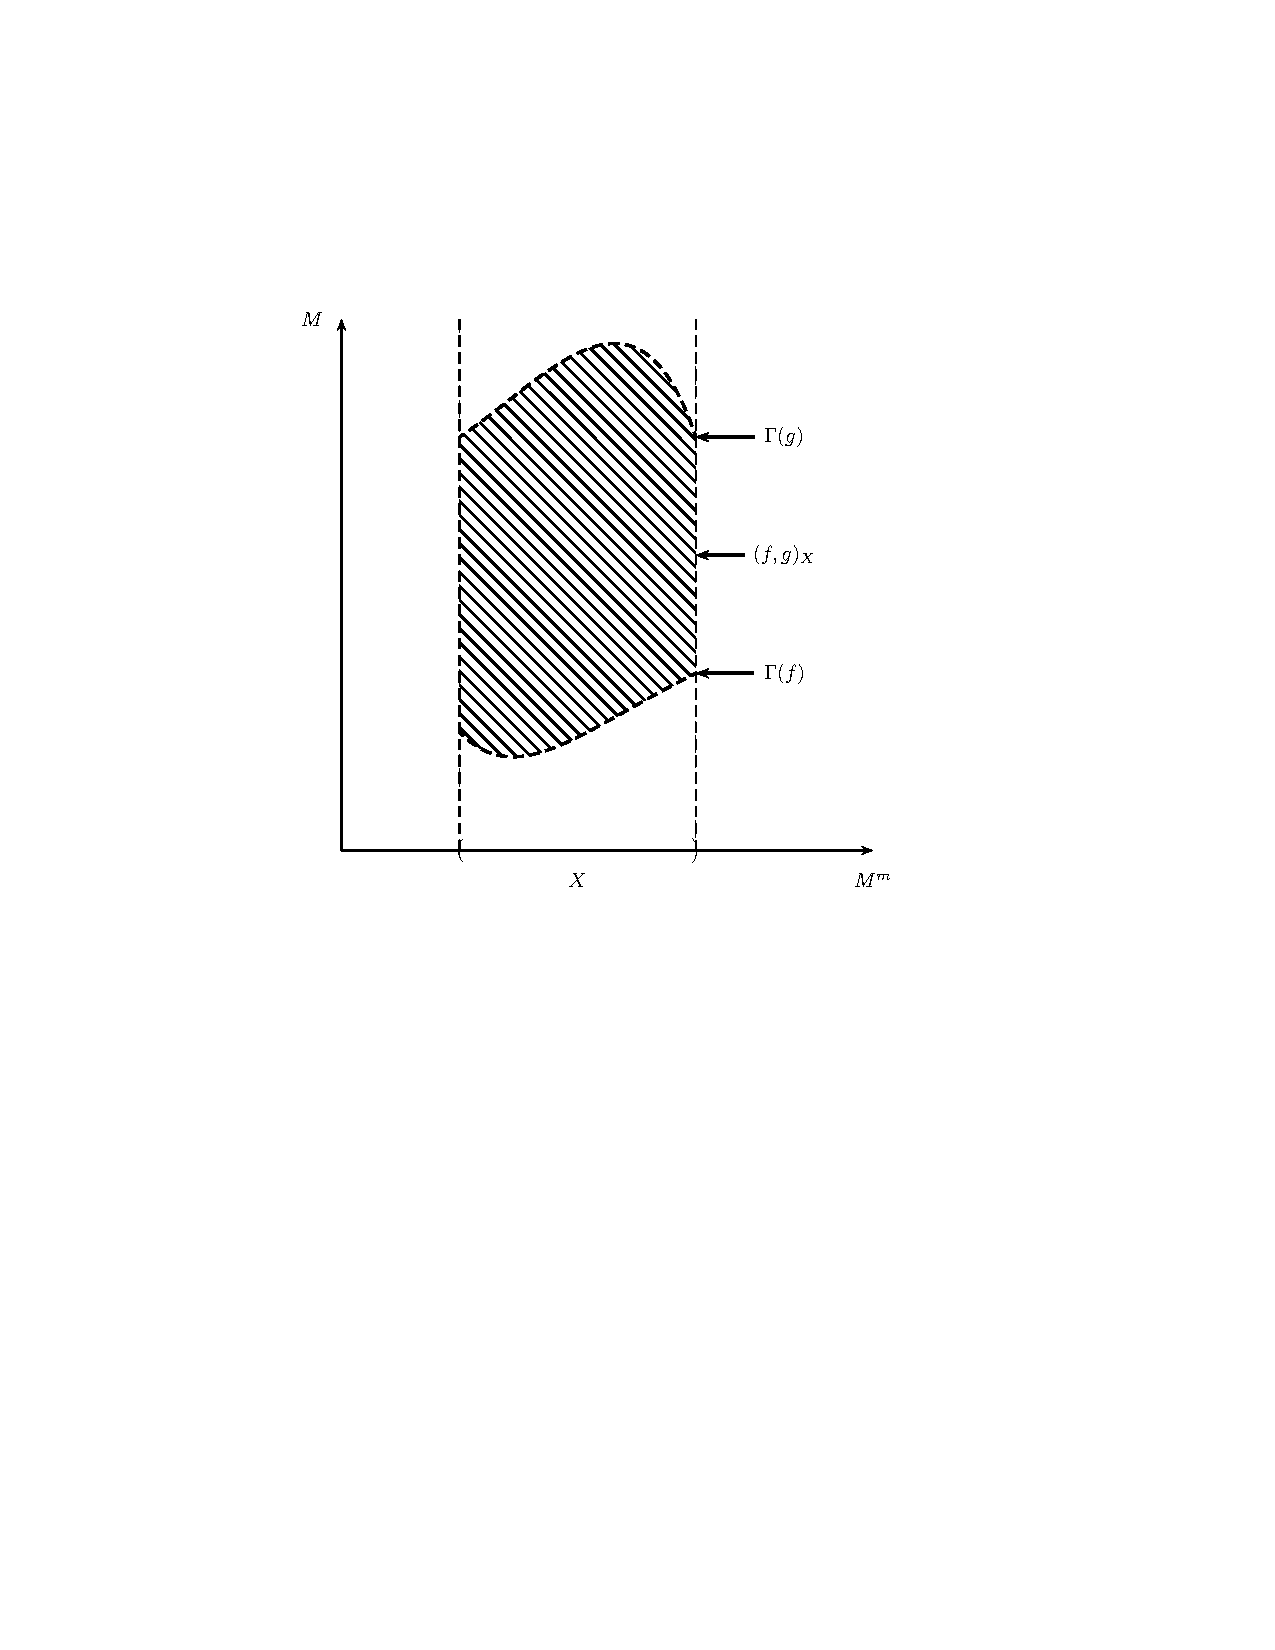
\includegraphics[height=5cm,width=4cm]{img/cell-.pdf}}


			\end{column}


		\end{columns}
\end{frame}

\begin{frame}[c]\frametitle{Decompositions}
    
	A \em decomposition \em of $M^n$ is a partition of $M^n$ into finitely many cells. It is defined recursively.

	\begin{itemize}
		\item A decomposition of $M$ is a collection,
		$$\{  (-\infty,a_1),(a_1,a_2),\ldots,(a_k,+\infty),\{a_1\},\ldots,\{a_k\} \}$$
		where $a_1<\ldots<a_k$ are points in $M$;
		\item a decomposition of $M^{n+1}$ is a finite partition of $M^{n+1}$ into cells $C$ s.t. the set of projections $\pi(C)$ is a decomposition of $M^n$.
	\end{itemize}

	A decomposition $\mathcal{D}$ of $M^n$ is said to \em partition \em a set $S \subseteq M^n$ if $S$ is a union of cells in $\mathcal{D}$.

\end{frame}

\begin{frame}[c]\frametitle{Cell Decomposition Theorem}
    
	\begin{beamerboxesrounded}[shadow=true]{Uniform Finiteness Property}
		Let $Y \subseteq M^{n+1}$ be definable and also for every $\bar{x} \in M^n$, 
		$$Y_{\bar{x}}:= \{  r \in M | (\bar{x},r) \in Y \}$$ is finite.
		Then there exists $N<\omega$ s.t. $Y_{\bar{x}} \leq N$ for all $\bar{x} \in M^n$.
	\end{beamerboxesrounded}

	\begin{beamerboxesrounded}[shadow=true]{Cell Decomposition Theorem}
		\begin{enumerate}
			\item Given any definable sets $A_1,\ldots,A_k\subseteq M^n$ there is a decomposition of $M^n$ partitioning each of $A_1,\ldots,A_k$.
			\item For each definable function $f:A \to M$, $A \subseteq M^n$, there is a decomposition $\mathcal{D}$ of $M^n$ partitioning $A$ s.t. the restriction $f|B:B\to M$ to each cell $B \in \mathcal{D}$ with $B\subseteq A$ is continuous.
		\end{enumerate}
	\end{beamerboxesrounded}

\end{frame}

\begin{frame}[c]\frametitle{Applications}
    
	\begin{beamerboxesrounded}[shadow=true]{Theorem}
		If $\mathcal{M}$ is an o-minimal structure, the $\text{Th}(\mathcal{M})$ is an o-minimal theory.
	\end{beamerboxesrounded}
	Proof...

\end{frame}

\subsection{Model Theory of o-Mininal Structures}

\begin{frame}[c]\frametitle{Prime models}
    
	\begin{beamerboxesrounded}[shadow=true]{Definition}
		Let $\mathcal{M}\vDash T$  and $A\subseteq \mathcal{M}$.
		$\mathcal{M}$ is said to be \em prime over $A$ \em if for any $\mathcal{M^{\prime}} \vDash T$ with
		$A \subseteq \mathcal{M^{\prime}}$, there is an elementary mapping $f:\mathcal{M} \to \mathcal{M^{\prime}}$ that is identity on $A$.
 	\end{beamerboxesrounded}

 	\begin{beamerboxesrounded}[shadow=true]{Theorem}
 		Let $A \subseteq \mathcal{M} \vDash T$, where $T$ is an o-minimal theory.
 		Then there is an a model $\mathcal{M^{\prime}} \vDash T$, $A \subseteq \mathcal{M^{\prime}}$
 		that is prime over $A$, and is unique up to isomorphism over $A$.
 	\end{beamerboxesrounded}

\end{frame}

\begin{frame}[c]\frametitle{Ressayre's Theorem}
    
	\begin{beamerboxesrounded}[shadow=true]{Definition}
		Let $\mathcal{M}$ be an $L$-structure and let $A\subseteq M$.
		Let $\delta$ be an ordinal and \break $(a_\alpha : \alpha < \delta)$ be a sequence of elements from $M$.
		Let $A_\alpha = A \cup \{a_\beta : \beta < \alpha \}$. 
		We call $(a_\alpha : \alpha < \delta)$ a \em construction \em over $A$ if $\text{tp}(a_\alpha / A_\alpha)$ is isolated for all $\alpha < \delta$.
	\end{beamerboxesrounded}

	\begin{beamerboxesrounded}[shadow=true]{Theorem [Ressayre]}
		Suppose that $A \subseteq \mathbb{M}$, $\mathcal{M}\prec \mathbb{M}$, $\mathcal{N}\prec \mathbb{M}$, and $\mathcal{M}$ and $\mathcal{N}$ are constructible over $A$.
		Then the identity map on $A$ extends to an isomorphism between $\mathcal{M}$ and $\mathcal{N}$.
	\end{beamerboxesrounded}

\end{frame}

\begin{frame}[t]\frametitle{Cuts and Noncuts}

	Let $\mathcal{M}\vDash T$. Let $p(x)\in S_1 (M)$.
	We say that $p(x)$ is a \em cut \em over $\mathcal{M}$ iff 
	there are non empty disjoint subsets $C_0$ and $C_1$ of $M$, s.t. $C_0 \cup C_1 = M$, 
	$C_0$ has no greatest element, $C_1$ has no least element, 
	for all $c\in C_0$, $``c<x"\in p(x)$, and for all $c\in C_1$, $``x<c"\in p(x)$.\\
	If $p(x)$ is not isolated and is not a cut, we call $p(x)$ a \em noncut\em.

	\begin{exampleblock}{Example}<2->

		Let $\tilde{\mathbb{Q}}$ be the field of real algebraic numbers. We know that 
		$\pi \in \mathbb{R} \backslash \tilde{\mathbb{Q}}$, so $\text{tp}(\pi,\tilde{\mathbb{Q}})$ 
		is a cut. \\
		If $t$ is an infinite hyperreal or $t$ is infinitesimally close to an element of 
		$\tilde{\mathbb{Q}}$, then $\text{tp}(t,\tilde{\mathbb{Q}})$ is a noncut. 

		\begin{overlayarea}{\textwidth}{2cm}
			\only<2>{\centering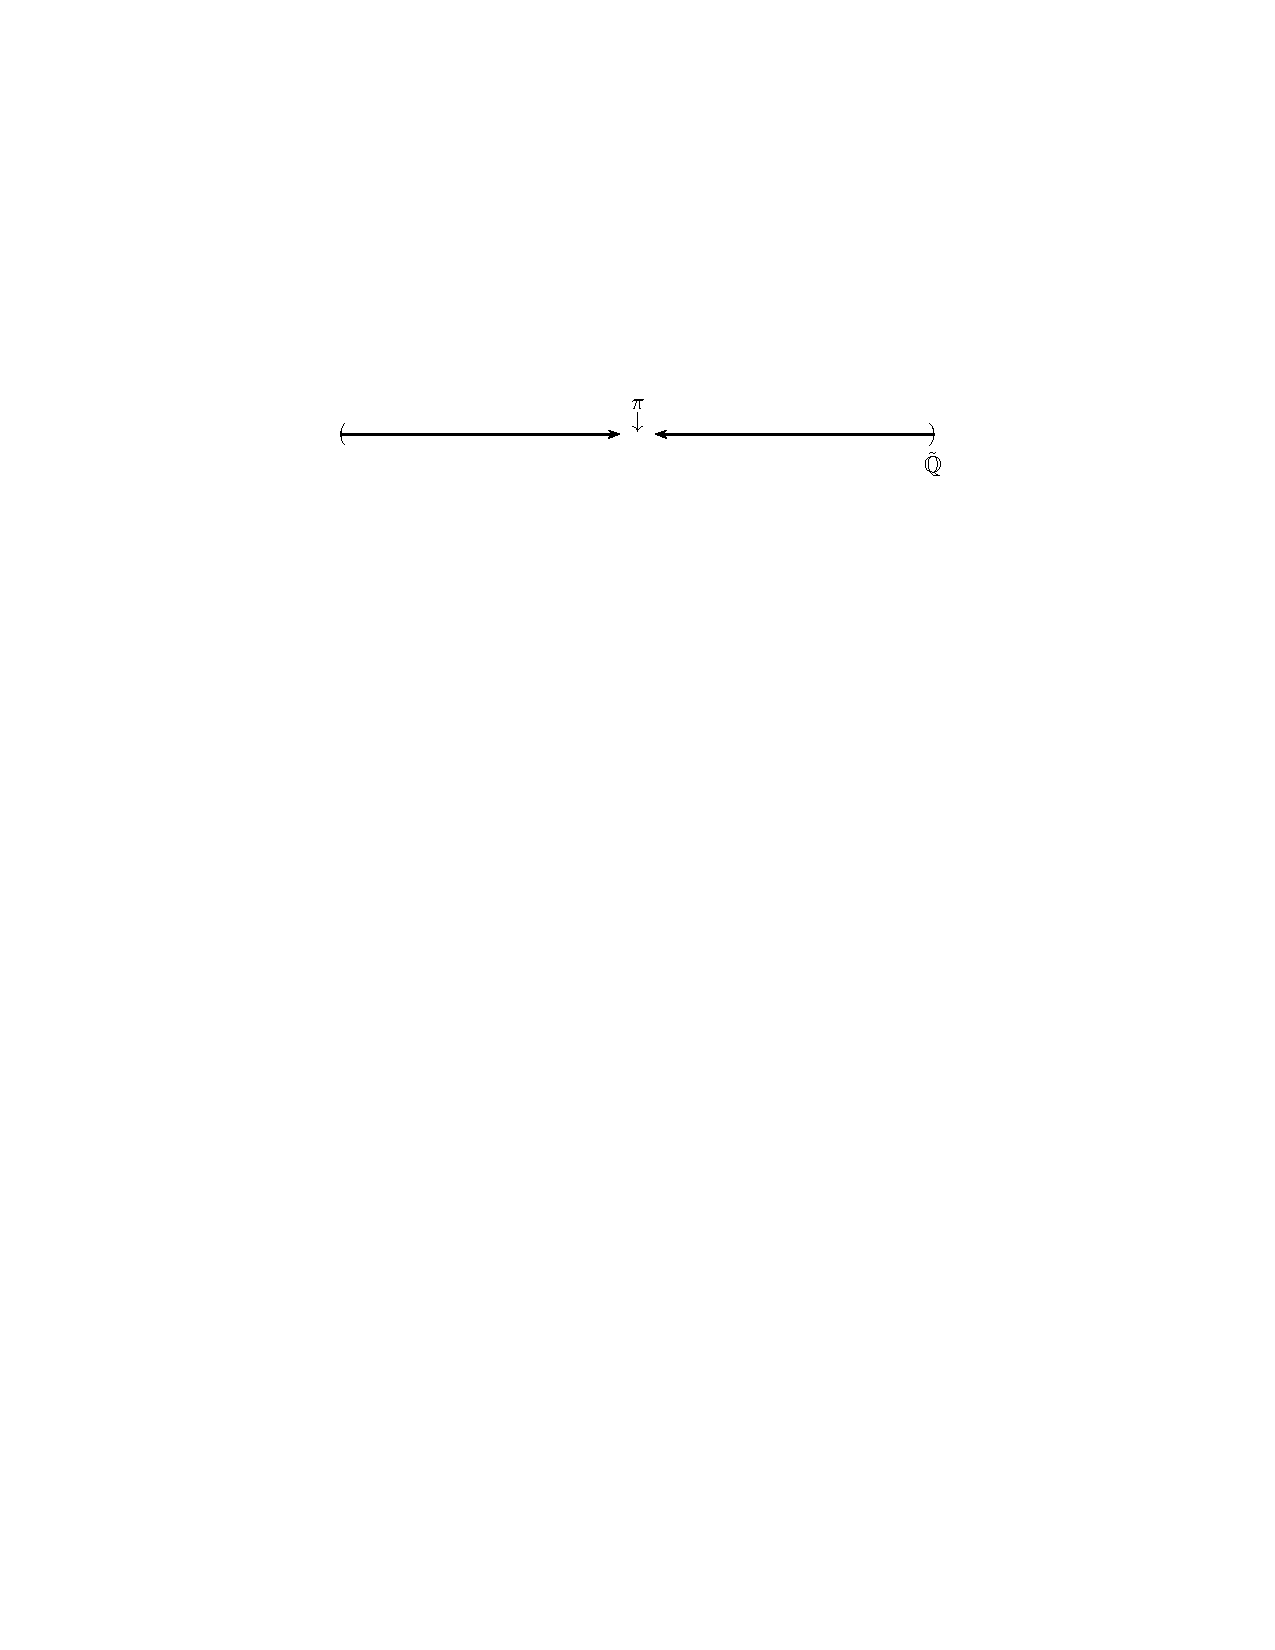
\includegraphics[height=1.5cm,width=11cm]{img/cut--.pdf}\par}
			\only<3>{\centering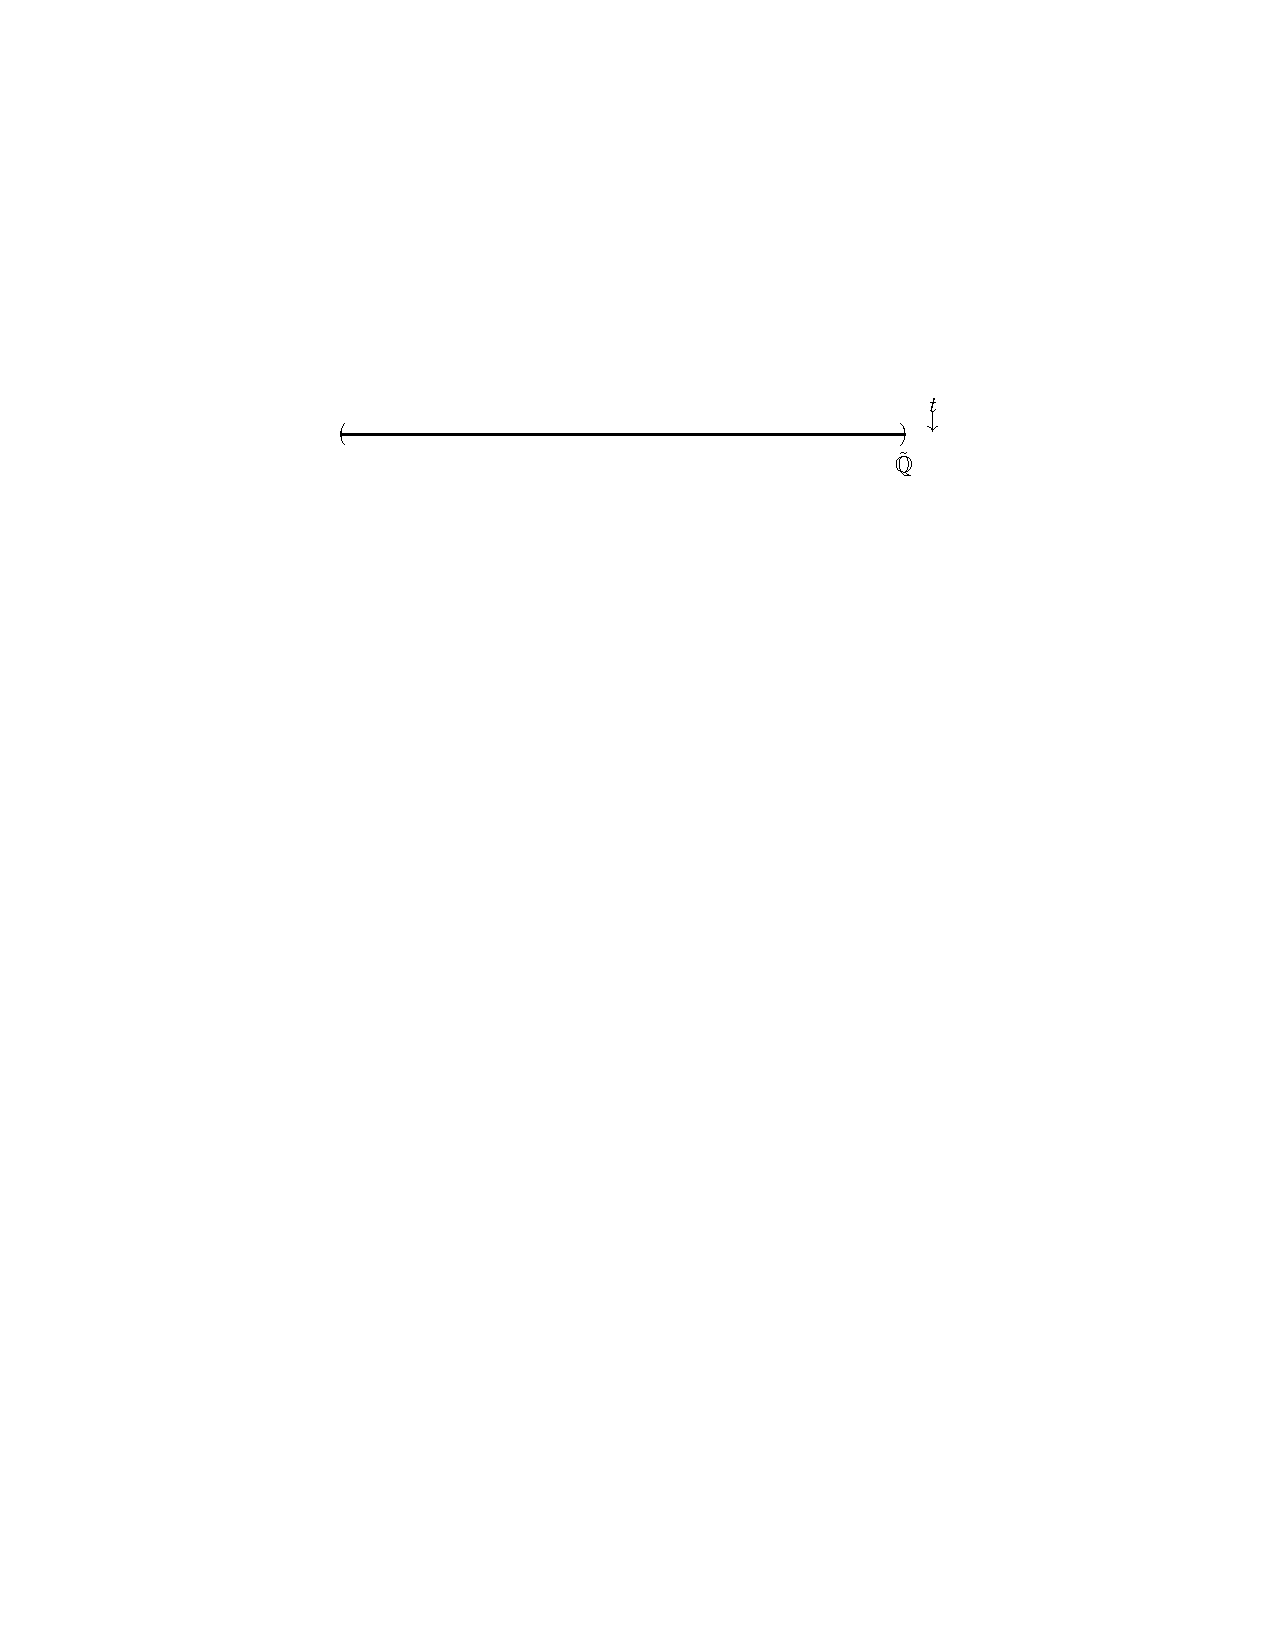
\includegraphics[height=1.5cm,width=11cm]{img/noncut1--.pdf}\par}
			\only<4>{\centering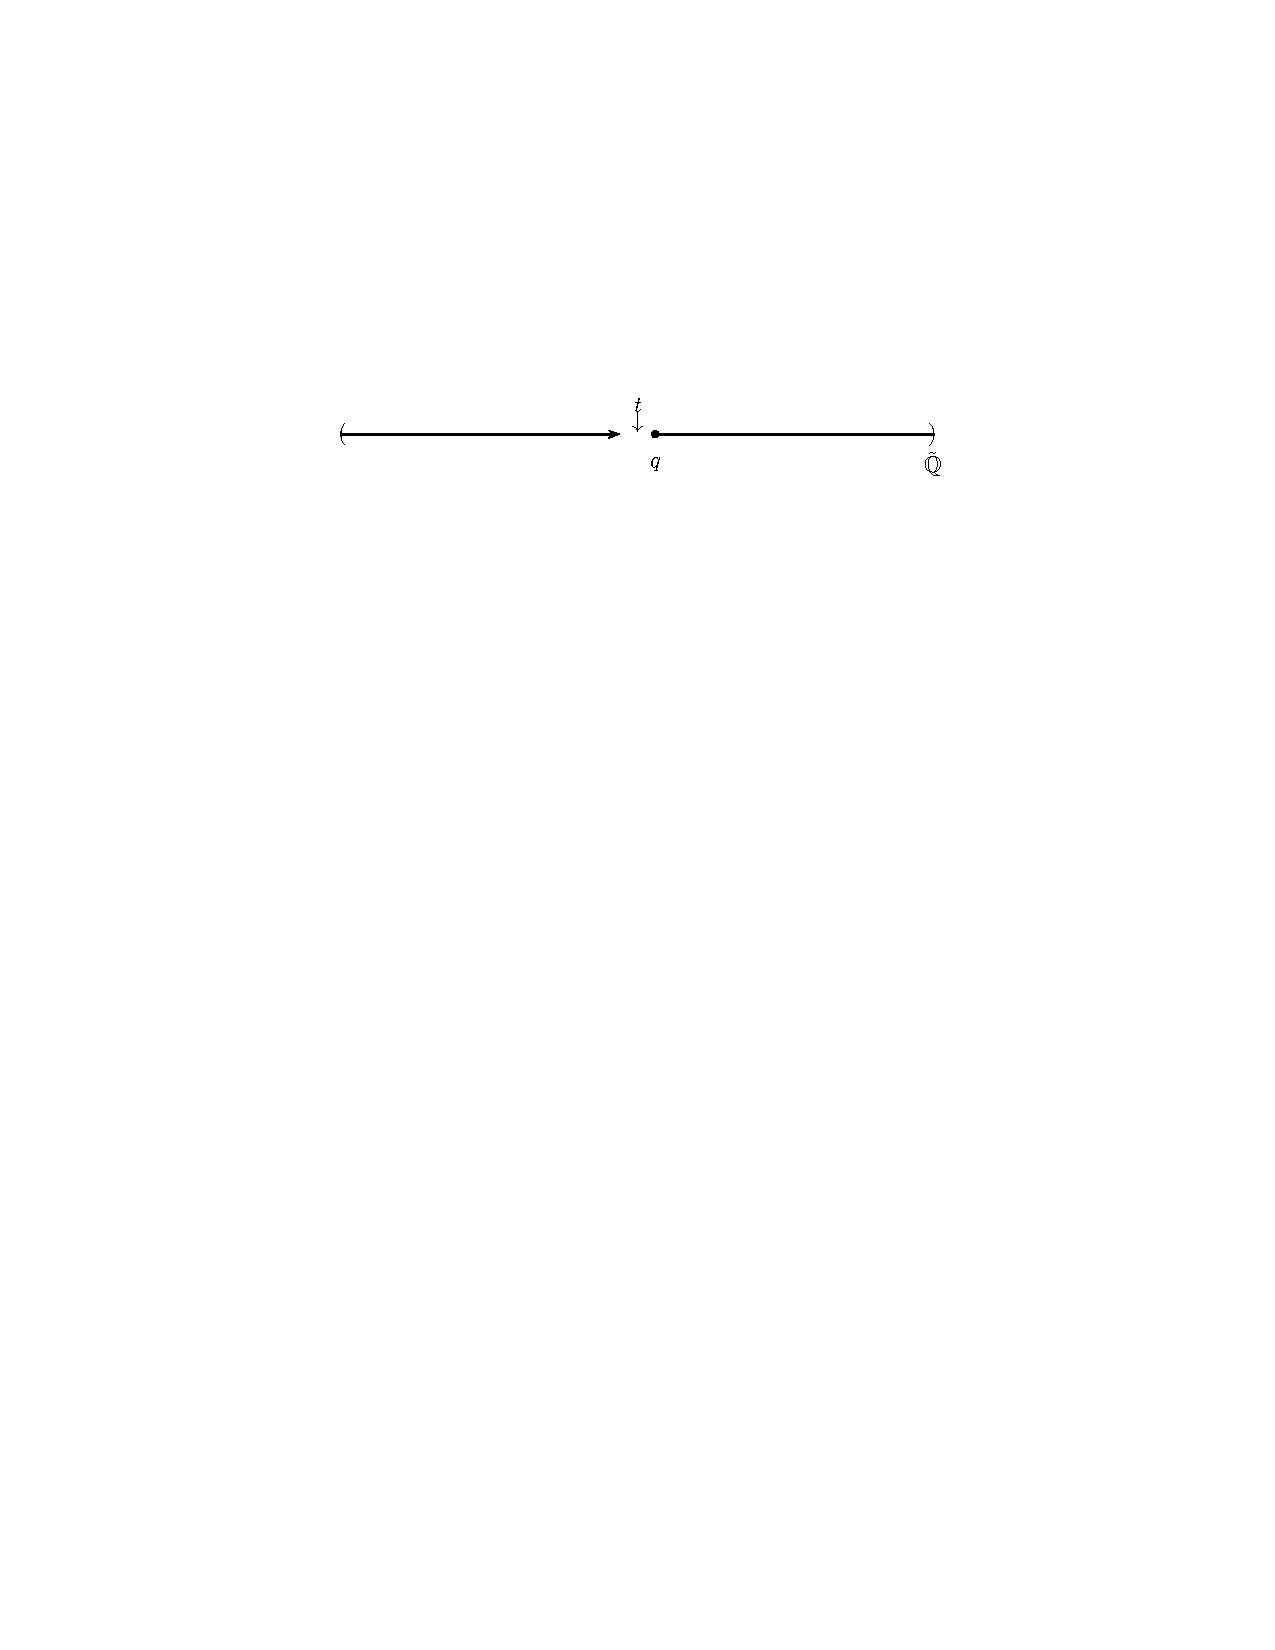
\includegraphics[height=1.5cm,width=11cm]{img/noncut2--.pdf}\par}
		\end{overlayarea}

	\end{exampleblock}

\end{frame}

\begin{frame}[c]\frametitle{Cuts and Noncuts}

	Let $\mathcal{M} \vDash T$, where $T$ is an o-minimal theory.
    \break
    \break
	\begin{beamerboxesrounded}[shadow=true]{Theorem}
		Let $\sigma (x) \in S_1 (M)$ be a cut. 
		Let $\tau (x) \in S_1 (M)$ be a noncut, and $b$ be a realization of $\tau (x)$.
		Then $\sigma (x)$ is omitted in $P(\mathcal{M} \cup \{b\})$.
	\end{beamerboxesrounded}

	\begin{beamerboxesrounded}[shadow=true]{Theorem}
		Let $\tau (x) \in S_1 (M)$ be a noncut. 
		Let $\sigma (x) \in S_1 (M)$ be a cut, and $b$ be a realization of $\sigma (x)$.
		Then $\tau (x)$ is omitted in $P(\mathcal{M} \cup \{b\})$.
	\end{beamerboxesrounded}

\end{frame}

\subsection{Groups and Fields}

\begin{frame}[t]\frametitle{Ordered Groups and Fields}
    
	\begin{beamerboxesrounded}[shadow=true]{Theorem}
		Let $\mathcal{G}=(G,+,0,<)$ be an o-minimal ordered group. 
		Then $\mathcal{G}$ is a divisible oredered abelian group.
	\end{beamerboxesrounded}

	\begin{beamerboxesrounded}[shadow=true]{Reminder}
		An abelian group $G$ is divisible if, for every positive integer $n$ and every $g \in G$, there exists $y \in G$ such that $ny = g$.
	\end{beamerboxesrounded}

	\begin{beamerboxesrounded}[shadow=true]{Theorem}
		Let $\mathcal{R}=(R,+,\cdot,1,<)$ be an o-minimal ordered ring. 
		Then $\mathcal{R}$ is a real closed field.
	\end{beamerboxesrounded}

	\begin{beamerboxesrounded}[shadow=true]{Reminder}
		A field $F$ is real closed if it is elementarily equivalent to $\mathbb{R}$.
	\end{beamerboxesrounded}

\end{frame}

\begin{frame}[t]\frametitle{Trichotomy Theorem}
    
	\begin{beamerboxesrounded}[shadow=true, upper=question]{Question}
		Is there a sense in which an o-minimal structure is either ``trivial'', or group-like, or field-like?
	\end{beamerboxesrounded}

	Any answer to this has to be ``local''.

	\begin{exampleblock}{Example}<2->

		\begin{itemize}
			\item $L$ is carrying the structure of a  pure dense linear order
			\item $M$ is carrying the structure of a  divisible abelian ordered group
			\item $R$ is carrying the structure of a  real closed field
		\end{itemize}

		\centering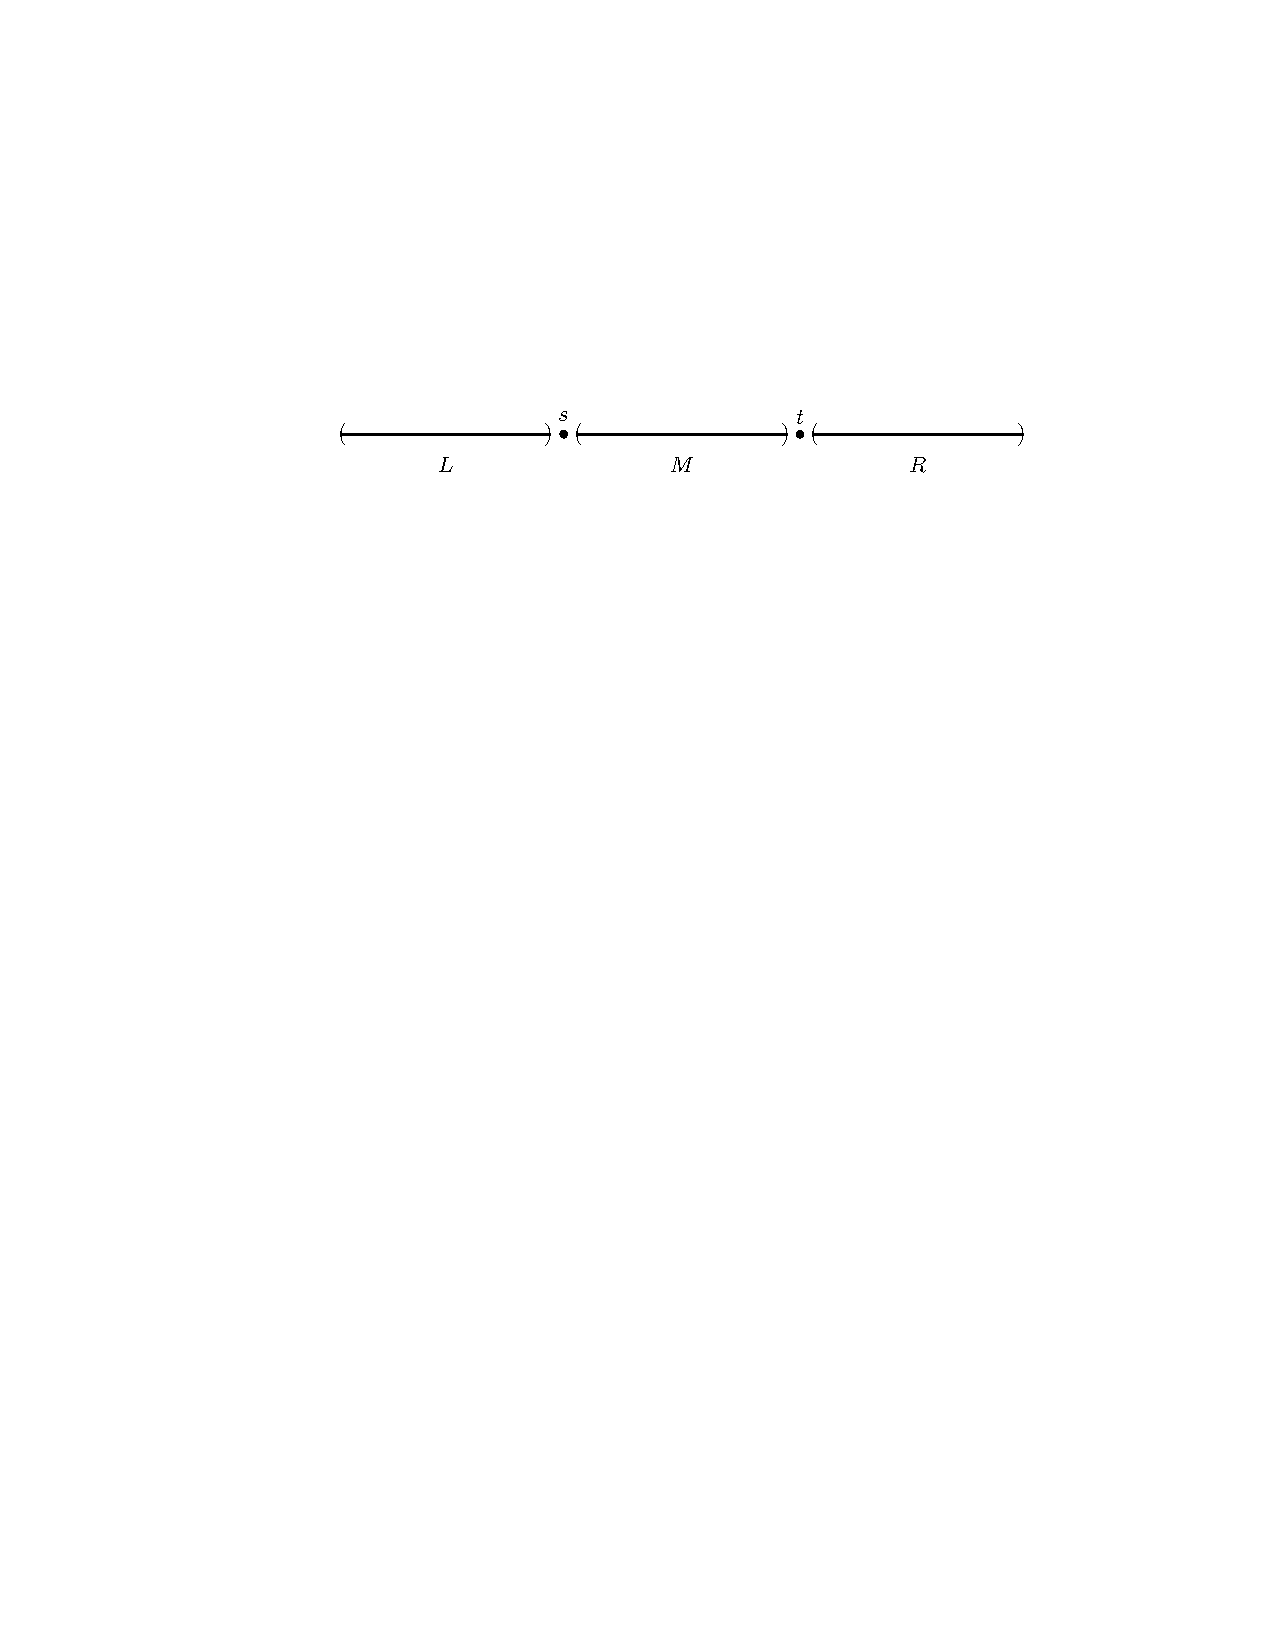
\includegraphics[height=1.25cm,width=12cm]{img/trichotomy--.pdf}\par

	\end{exampleblock}

\end{frame}

\begin{frame}[c]\frametitle{Trichotomy Theorem}
    
	\begin{beamerboxesrounded}[shadow=true]{Trichotomy Theorem}
		
		Let $\mathcal{M}$ be a sufficiently saturated o-minimal structure.
		Given an $a \in M$ one and only one of the following holds,

		\begin{itemize}
			\item $a$ is trivial,
			\item the structure that $\mathcal{M}$ induces on some convex neighborhood of $a$ is an ordered vector space over an ordered division ring.
			\item the structure that $\mathcal{M}$ induces over some open interval around $a$ is an o-minimal expansion of a real closed field.
		\end{itemize}

	\end{beamerboxesrounded}

\end{frame}
%!TEX root = main.tex

\section{Variations}
\subsection{Weak o-minimality}

\begin{frame}[c]\frametitle{Weakly o-minimal structures}
	
	Let $\mathcal{M} = (M,<, \dots )$ be a linearly ordered structure.
    
	\begin{beamerboxesrounded}[shadow=true]{Definition}
		A set $C \subseteq M$ is called \em convex \em, if for any $a,b \in C$ with $a<b$, and $c\in M$ such that $a<c<b$, then $c \in C$. 
	\end{beamerboxesrounded}

	\begin{beamerboxesrounded}[shadow=true]{Definition}
		A structure $\mathcal{M}$ will be called \em weakly o-minimal \em, if the definable subsets of $\mathcal{M}$ are finite unions of convex sets in $(M,<)$.\\
		We say that a complete theory $T$ is \em weakly o-minimal \em if every model of $T$ is weakly o-minimal. 
	\end{beamerboxesrounded}

	\begin{beamerboxesrounded}[shadow=true]{Theorem}
		Expanding an o-minimal structure with unary predicates for convex subsets yields a structure with weakly o-minimal theory.
	\end{beamerboxesrounded}

\end{frame}

\begin{frame}[t]\frametitle{Monotonicity}
    \only<1>{
		Let $\mathcal{M}=(M,<,P,Q,f)$ such that.
		\begin{itemize}
			\item $M$ is the disjoint union of the interpretations of the unary relations $P$ and $Q$
			\item $P$ is the interpretation of $\mathbb{Q}$ with the usual order
			\item $Q$ is the interpretation of $\mathbb{Q} \times \mathbb{Q}$, lexicographically ordered
			\item $P$ proeceds $Q$ in $<$ on $M$ 
			\item $f:Q \to P$, $f((n,m))=n$ for all $n,m \in \mathbb{Q}$
		\end{itemize}
		$M$ is weakly o-minimal and also $\text{Th}(\mathcal{M})$ is weakly o-minimal.\\~\\
		}
	\only<2>{
		\begin{center}
			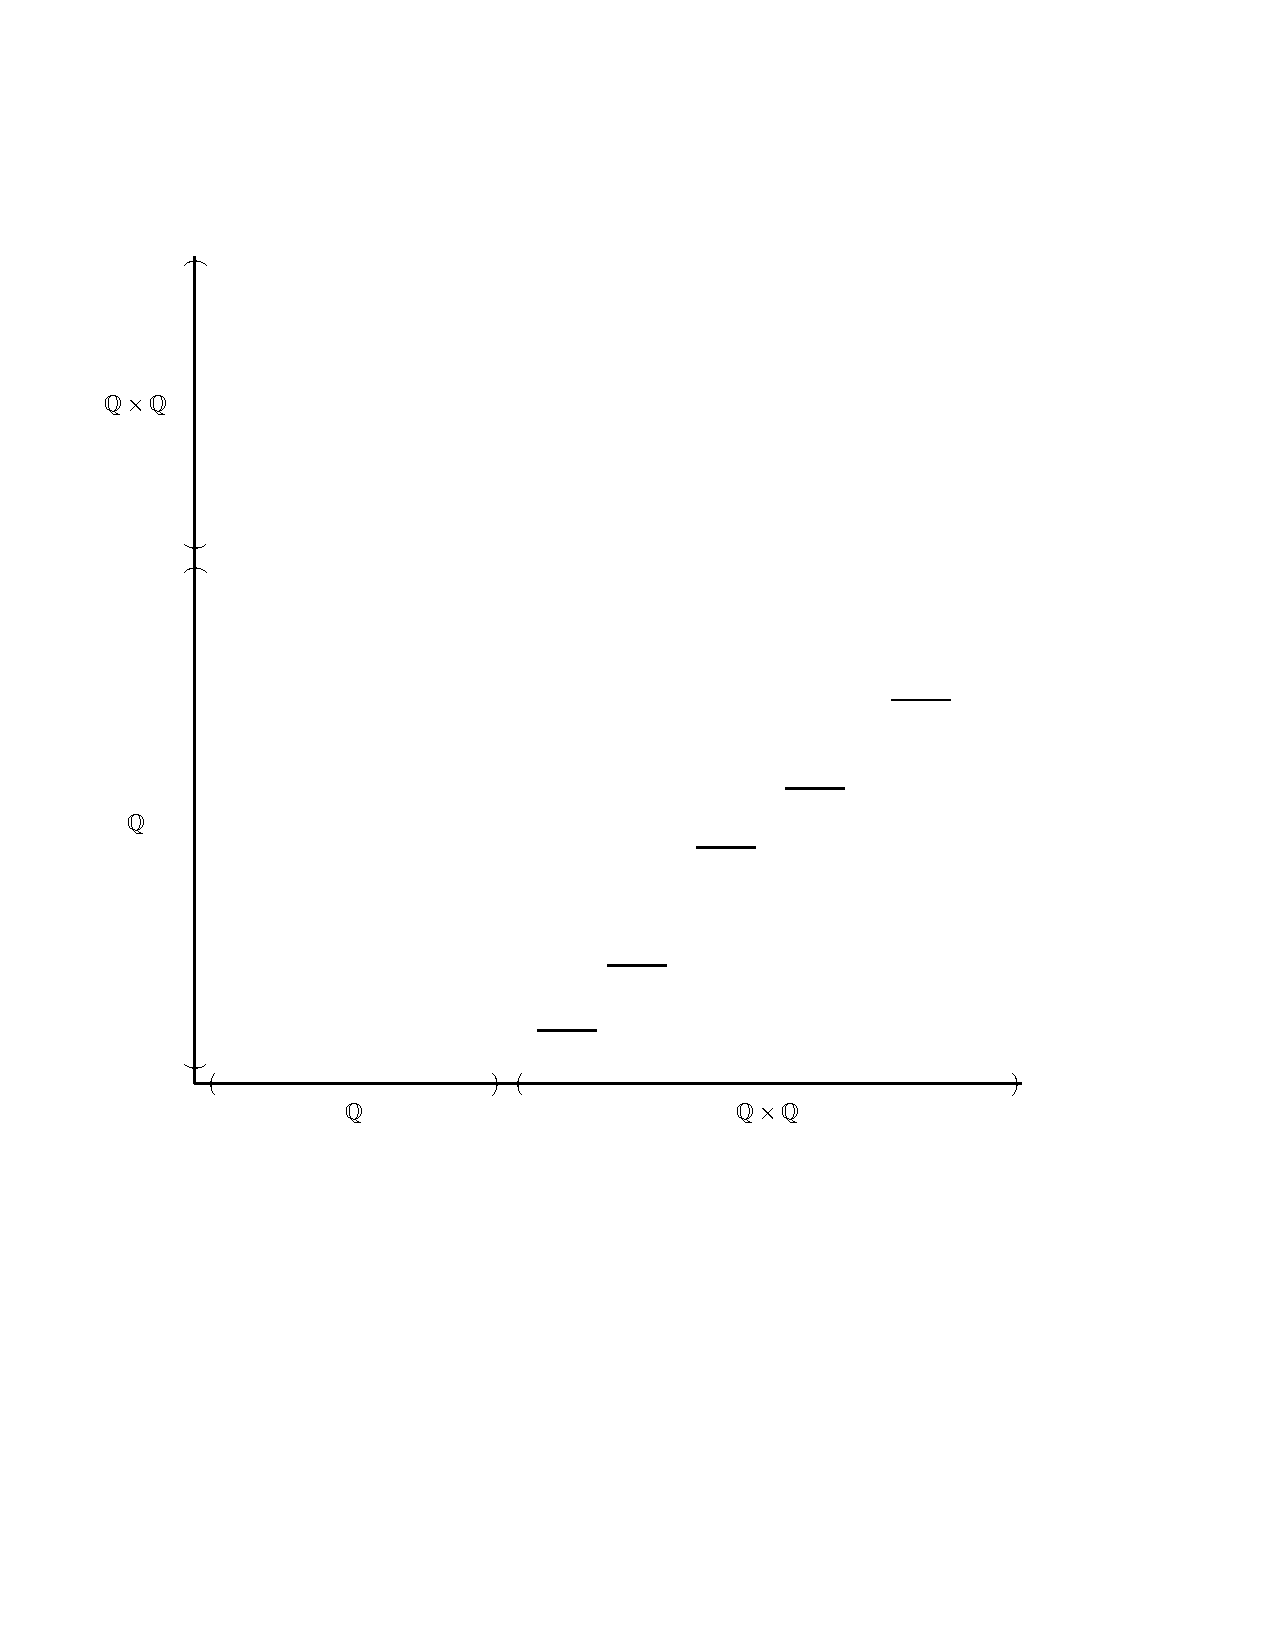
\includegraphics[height=7cm,width=7cm]{img/weakly-monotonicity--.pdf}
		\end{center}
	}

\end{frame}

\begin{frame}[t]\frametitle{Weakly o-minimal structures}

    
	\begin{itemize}
		\item[$\color{darkred}\bigstar$] We have a local monotonicity theorem. \citep{arefiev1997monotonicity}
		\item[$\color{darkred}\bigstar$] Weakly o-minimal structures do not neccesserily have weakly o-minimal theory.
		\item[$\color{darkred}\bigstar$] Weakly o-minimal structures do not neccesserily have prime models.
	\end{itemize}

	\begin{beamerboxesrounded}[shadow=true]{Theorem \citep{macpherson2000weakly}}
		Every weakly o-minimal ordered group is divisible and abelian.
	\end{beamerboxesrounded}

	\begin{beamerboxesrounded}[shadow=true]{Theorem \citep{macpherson2000weakly}}
		Every weakly o-minimal ordered field is real closed.
	\end{beamerboxesrounded}
\end{frame}

\subsection{Other variations}

\begin{frame}[t]\frametitle{A definition for minimality}
    
	Let $L\subset L^{+}$ be languages, and $\mathcal{K}$ be an elementary 
	class of $L$-structures.\\~\\
	\begin{beamerboxesrounded}[shadow=true]{Definition \citep{macpherson1996variants}}
		An $L^{+}$-structure $\mathcal{M}$ is \em $\mathcal{K}$-minimal \em if the 
		the reduct $\mathcal{M}|_{L}$ is in $\mathcal{K}$ and every $L^{+}$-definable subset of $M$ is definable by a quantifier-free $L$-formula.\\
		A complete $L^{+}$-theory is \em $\mathcal{K}$-minimal \em if all its models are $\mathcal{K}$-minimal.
	\end{beamerboxesrounded}

	\begin{itemize}
		\item[$\color{darkred}\bigstar$] o-minimality is a special case of the above definition but not weak o-minimality.
		\item[$\color{darkred}\bigstar$] $\mathcal{K}$-minimality is closed under reducts to languages containg $L$, and under expansion by constants.
	\end{itemize}

\end{frame}

\begin{frame}[t]\frametitle{C-minimality}
    
	Let $C(x;y,z)$ be a ternary realation, $L=\{ C \}$, and $\mathcal{K}_{C}$ 
	be the class of $L$-structures satisfying the following axioms.

	\begin{itemize}
		\item $(\forall xyz)[C(x;y,z)\to C(x;z,y)]$
		\item $(\forall xyz)[C(x;y,z)\to C(y;x,z)]$
		\item $(\forall xyzw)[C(x;y,z)\to (C(w;y,z) \vee C(x;w,z))]$
		\item $(\forall xy)[x\neq y \to (\exists z \neq y)C(x;y,z)]$
		\item $(\exists xy)(x\neq y)$
	\end{itemize}

	\begin{beamerboxesrounded}[shadow=true]{Definition}
		A structure $\mathcal{M}=(M,C,\ldots)$ is \em $C$-minimal \em if 
		its theory is $\mathcal{K}_{C}$-minimal.
	\end{beamerboxesrounded}

\end{frame}

\begin{frame}[t]\frametitle{P-minimality}
    
	\begin{beamerboxesrounded}[shadow=true]{Definition}
		Let $L=(+,-,\cdot,0,1,(P_{n})_{n>1})$, where $P_n$ are unary
		predicates. Regard $\mathbb{Q}_p$ as an $L$-structure, letting $P_n$ picking the $n^{\text{th}}$ powers in $\mathbf{Q_p}$.
		Let $\mathcal{K}_P$ be the class of $L$-structures elementarily equivalent to $\mathbb{Q}_p$. 
		Then if $L^{+}\supseteq L$, an $L^{+}$-structure is \em $P$-minimal \em
		if all models of its theory are $\mathcal{K}_P$-minimal
	\end{beamerboxesrounded}

\end{frame}
%!TEX root = main.tex

\section{Summary}

\begin{frame}[c]\frametitle{Summary}
    
	\begin{center}
		\begin{tabulary}{\textwidth}{ | C | C | C | C | C |}
			\hline
				      			& \small{o-minimal}	& \small{weakly} 		  & \small{$C$-minimal}		& \small{$P$-minimal}	  	\\ \hline
			\small{Monotonicity}& \ding{51}   		& local				  	  &	\ding{51}				& \ding{51}					\\ \hline
			CDT					& \ding{51}			& \ding{51}			  	  & \ding{51}				& \tiny{iff it has Skolem functions}			\\ \hline
			Prime Model			& \ding{51}			& \ding{55}			  	  & \ding{55}				& \ding{55}					\\ \hline
			Groups				& DAG		 		& DAG				  	  & 						& 							\\ \hline
			Fields				& RCF				& RCF				  	  & ACVF					& 							\\ \hline
			Exchange			& \ding{51}			& \ding{55}			  	  & \ding{55}				& \ding{51}					\\ \hline
			IP					& \ding{55}			& \ding{55}			  	  & \ding{55}				& \ding{55}					\\ \hline
		\end{tabulary}
	\end{center}

\end{frame}

\end{document}